% chapters/hbm.tex
%
% Copyright 2022 Alexander Lyttle.
%
% This work may be distributed and/or modified under the conditions of the
% LaTeX Project Public License (LPPL) version 1.3 or later.
%
% The latest version of this license is in
% https://www.latex-project.org/lppl.txt and version 1.3 or later is part of
% all distributions of LaTeX version 2005/12/01 or later.
%
%
\chapter{Hierarchical Bayesian Models}

We observe apparent visual magnitude (\(v_i\)) and dimensionless parallax (\(\varpi_i\)) of \(i= 1,\dots,N_\mathrm{stars}\) stars each at some dimensionless distance (\(d_i\)) from the observer. Each observable is measured independently with Gaussian noise characterised by \(\sigma_{v,i} = 0.1\) and \(\sigma_{\varpi,i} = 0.01\) respectively.

%
\begin{equation}
    v_i = V_i + 5 \log_{10} d_i,
\end{equation}
%

\begin{figure}[!tb]
    \centering
    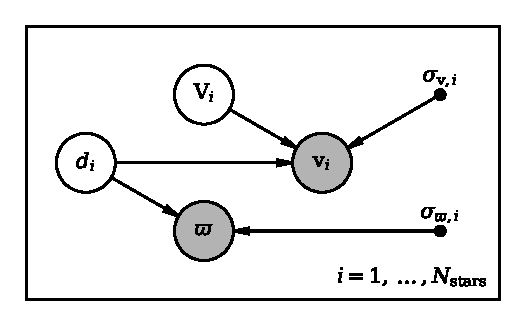
\includegraphics{figures/simple-pgm.pdf}
    \caption{Simple.}
\end{figure}

Bayes' theorem,
%
\begin{equation}
    p(d_i, V_i \mid \varpi_i, v_i) \propto p(\varpi_i, v_i \mid d_i, V_i) \, p(d_i, V_i)
\end{equation}
%

\begin{figure}[!tb]
    \centering
    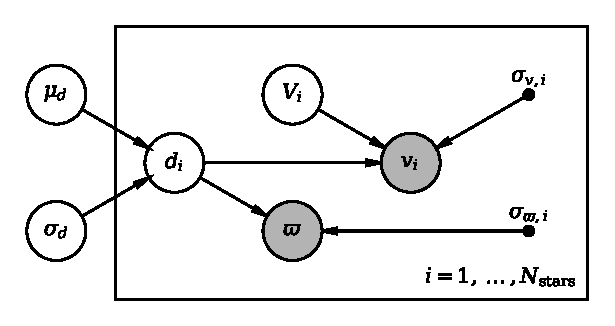
\includegraphics{figures/hbm-pgm.pdf}
    \caption{HBM.}
\end{figure}

Hierarchical, we assume that the model parameters depend on population-level parameters,
%
\begin{equation}
    p(\mu_d, \sigma_d, \vect{d}, \vect{V} \mid \vect{\varpi}, \vect{v}) \propto p(\vect{\varpi}, \vect{v} \mid \vect{d}, \vect{V}) \, p(\vect{d} \mid \mu_d, \sigma_d) \, p(\mu_d, \sigma_d, \vect{V})
\end{equation}
%

We assume \(d_i \sim \mathcal{N}(\mu_d, \sigma_d^2)\).

Maybe just do the partially-pooled case and say that the max-pooled is good when we know the parameter follows some absolute law.

\begin{figure}[p]
    \centering
    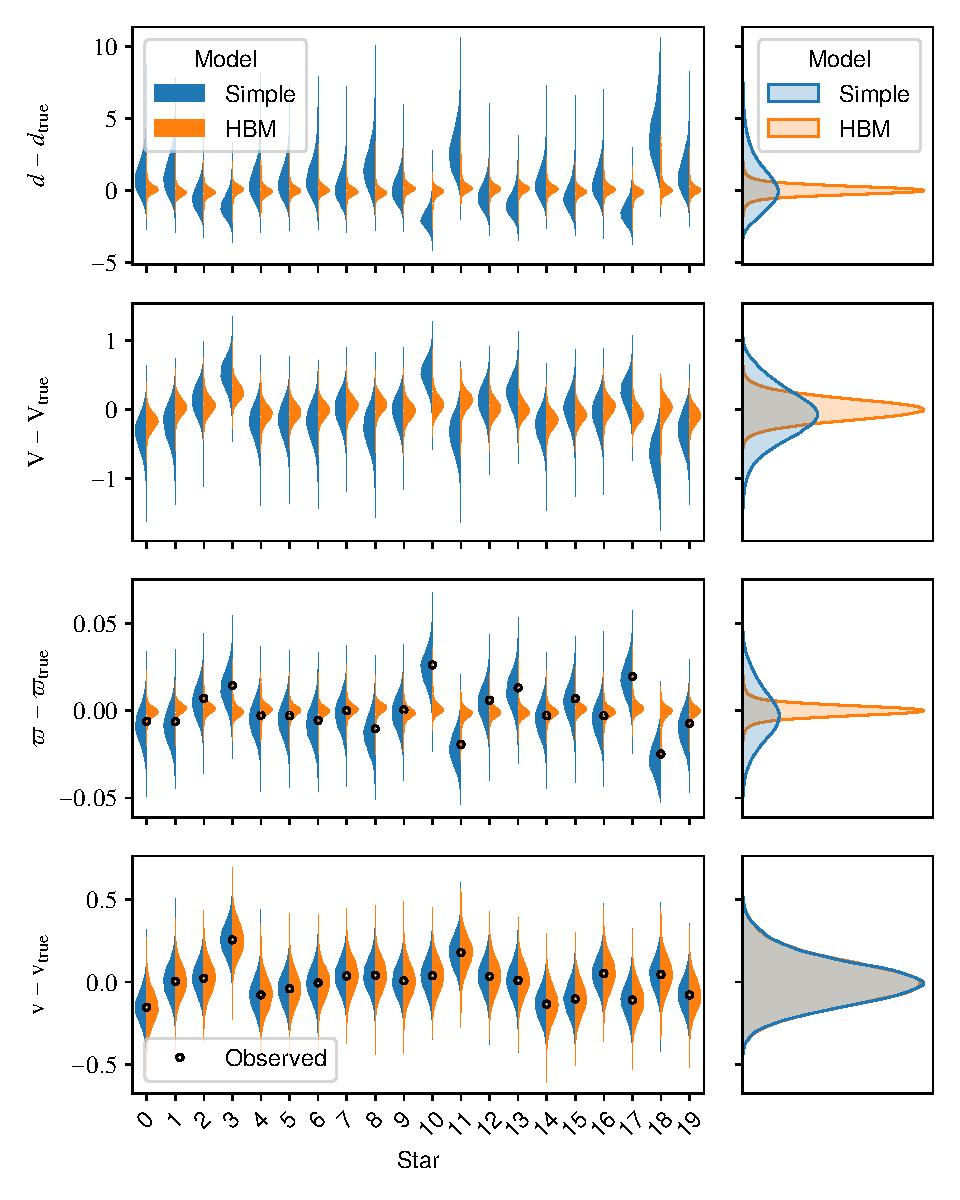
\includegraphics{figures/hbm-results.pdf}
    \caption{Results.}
\end{figure}